\documentclass[a4paper,11pt]{article}
\usepackage{amsmath,amsthm,amsfonts,amssymb,amscd,amstext,vmargin,graphics,graphicx,tabularx,multicol} \usepackage[french]{babel}
\usepackage[utf8]{inputenc}  
\usepackage[T1]{fontenc} 
\usepackage[T1]{fontenc}
\usepackage{amsmath,amssymb}
\usepackage{pstricks-add,tikz,tkz-tab,variations}
\usepackage[autolanguage,np]{numprint} 
\usepackage{color}
\usepackage{ulem}


\setmarginsrb{1.5cm}{0.5cm}{1cm}{0.5cm}{0cm}{0cm}{0cm}{0cm} %Gauche, haut, droite, haut
\newcounter{numexo}
\newcommand{\exo}[1]{\stepcounter{numexo}\noindent{\bf Exercice~\thenumexo} : \marginpar{\hfill /#1}}
\reversemarginpar


\newcounter{enumtabi}
\newcounter{enumtaba}
\newcommand{\q}{\stepcounter{enumtabi} \theenumtabi.  }
\newcommand{\qa}{\stepcounter{enumtaba} (\alph{enumtaba}) }
\newcommand{\initq}{\setcounter{enumtabi}{0}}
\newcommand{\initqa}{\setcounter{enumtaba}{0}}

\newcommand{\be}{\begin{enumerate}}
\newcommand{\ee}{\end{enumerate}}
\newcommand{\bi}{\begin{itemize}}
\newcommand{\ei}{\end{itemize}}
\newcommand{\bp}{\begin{pspicture*}}
\newcommand{\ep}{\end{pspicture*}}
\newcommand{\bt}{\begin{tabular}}
\newcommand{\et}{\end{tabular}}
\renewcommand{\tabularxcolumn}[1]{>{\centering}m{#1}} %(colonne m{} centrée, au lieu de p par défault) 
\newcommand{\tnl}{\tabularnewline}

\newcommand{\trait}{\noindent \rule{\linewidth}{0.2mm}}
\newcommand{\hs}[1]{\hspace{#1}}
\newcommand{\vs}[1]{\vspace{#1}}

\newcommand{\N}{\mathbb{N}}
\newcommand{\Z}{\mathbb{Z}}
\newcommand{\R}{\mathbb{R}}
\newcommand{\C}{\mathbb{C}}
\newcommand{\Dcal}{\mathcal{D}}
\newcommand{\Ccal}{\mathcal{C}}
\newcommand{\mc}{\mathcal}

\newcommand{\vect}[1]{\overrightarrow{#1}}
\newcommand{\ds}{\displaystyle}
\newcommand{\eq}{\quad \Leftrightarrow \quad}
\newcommand{\vecti}{\vec{\imath}}
\newcommand{\vectj}{\vec{\jmath}}
\newcommand{\Oij}{(O;\vec{\imath}, \vec{\jmath})}
\newcommand{\OIJ}{(O;I,J)}

\newcommand{\bmul}[1]{\begin{multicols}{#1}}
\newcommand{\emul}{\end{multicols}}


\newcommand{\reponse}[1][1]{%
\multido{}{#1}{\makebox[\linewidth]{\rule[0pt]{0pt}{20pt}\dotfill}
}}

\newcommand{\titre}[5] 
% #1: titre #2: haut gauche #3: bas gauche #4: haut droite #5: bas droite
{
\noindent #2 \hfill #4 \\
#3 \hfill #5

\vspace{-1.6cm}

\begin{center}\rule{6cm}{0.5mm}\end{center}
\vspace{0.2cm}
\begin{center}{\large{\textbf{#1}}}\end{center}
\begin{center}\rule{6cm}{0.5mm}\end{center}
}



\begin{document}
\pagestyle{empty}
\titre{Correction du contrôle 2 : Calcul littéral, théorème de Pythagore et trigonométrie}{3 ème}{}{}{}


\exo{2}

\initq \q Développer et réduire $M = (9 - x)(2x + 6) - 3 (x - 4)$.  \\

\red $M = (9 - x)(2x + 6) - 3 (x - 4)$\\

$M = 18x + 54 - 2x^{2} -6x - 3 (x - 4)$\\

$M = 18x + 54 - 2x^{2} -6x - 3x + 12$\\

\fbox{$M = - 2x^{2} + 9x + 66$}\\


\black \q Calculer l'expression M pour $x=0$.\\

\red Grâce à la question précédente, on sait que $M = (9 - x)(2x + 6) - 3 (x - 4)$ ou $M = - 2x^{2} + 9x + 66$ \\

On préfèrera choisir la deuxième expression pour calculer avec $x=0$ :\\

$M = - 2\times 0^{2} + 9 \times 0 + 66$ donc \fbox{$M= 66$}\\




\black \exo{2}

\initq \q Développer et réduire $K = (2x + 1)(2x - 1)$.\\

\red $K = (2x + 1)(2x - 1)$\\

$K = 4x^{2} - 2x + 2x -1$\\

\fbox{$K= 4x^{2} - 1$}\\


\black \q En déduire le résultat de la multiplication suivante : $20 001 \times 19 999$. (\textbf{Justifier votre réponse avec la question précédente.}\\

\red $20 001 \times 19 999 = (\nombre{20 000} + 1)(\nombre{20 000} - 1) = (2 \times \nombre{10 000} + 1)(2 \times \nombre{10 000} - 1) $ d'après la question précédente\\

$\nombre{20 001} \times \nombre{19 999} = 4 \times \nombre{10 000}^{2} - 1 $\\
$\nombre{20 001} \times \nombre{19 999} = 4 \times \nombre{100 000 000} - 1$\\
$\nombre{20 001} \times \nombre{19 999} = \nombre{400 000 000} - 1$\\
$\nombre{ 20 001} \times \nombre{19 999} = \nombre{399 999 999}$\\

\black \exo{3} Factoriser les expressions suivantes : 

\bmul{2}

\black $H = 24x^{3} - 8x + 16 x^{2}$\\

\red $H = 8x (3x^{2} - 1 + 2x)\\ $

\black $ E = (4 + x)^{2} - (4 + x)(3x + 1)$\\

\red $ E = (4 + x)(4 + x) - (4 + x)(3x + 1)$\\

$ E = (4 + x)[(4 + x) - (3x + 1)]$\\

$ E = (4 + x)(4 + x - 3x - 1)$\\

$ E = (4 + x)(3 - 2x)$\\



\columnbreak

\black $S = 12xy + 3y^{2}$\\

\red $S = 3y (4x+ y)$\\

\black $Z = (2x - 3)(6 - x) + (3x - 2)(2x - 3)$\\

\red $Z = (2x - 3)[(6 - x) + (3x - 2)]$\\

$Z = (2x - 3)[6 - x + 3x - 2]$\\

$Z = (2x - 3)(4 + 2x )$\\
 

\emul



\exo{2} Pour chacune des questions, entourer en bleu la bonne réponse :

\bmul{2}

\red Question 1 : La réponse est 9 \\

Question 2 : La réponse est $-6x^{2} + 11x -3$\\

\columnbreak

Question 3 : $sin \widehat{a} = 0,8$\\

Question 4 : $tan \widehat{a} = \dfrac{5}{12}$\\

\emul


\black \exo{5}

RST est un triangle tel que RS = 6,4 cm, ST = 8 cm et RT = 4,8 cm.\\

\initq \q Construire le triangle en vraie grandeur puis montrer qu'il est rectangle en R.\\

\red Dans le triangle RST, la plus grande longueur est ST = 8cm.\\

\bmul{2}
D'une part, $ST^{2} = 8^{2} $\\
Donc  $ST^{2} = 64$\\


\columnbreak

D'autre part, $RS^{2} + RT^{2} = 6,4^{2} + 4,8^{2}$\\
Donc $RS^{2} + RT^{2} = 40,96 + 23,04 = 64$\\
\emul

Ainsi, comme on vient de prouver que  $RS^{2} + RT^{2} = ST^{2}$, d'après la réciproque du théorème de Pythagore, on peut affirmer que le triangle RST est rectangle en R.\\



\black \q  Calculer la valeur arrondie au degré près de la mesure de l'angle $\widehat{RST}$. En déduire la mesure de l'angle $\widehat{RTS}$\\

\red 
\underline{Calcul de l'angle $\widehat{RST}$ : }

Dans le triangle RST rectangle en R. On cherche la mesure de l'angle $\widehat{RST}$ et on connaît la mesure de son côté opposé [RT] et celle de son côté adjacent [SR].\\

On utilise la formule de la tangente :\\

$ tan \widehat{RST} = \dfrac{RT}{RS}$\\

$ tan \widehat{RST} = \dfrac{4,8}{6,4}$\\

A l'aide de la calculatrice, je trouve la valeur de l'angle : \fbox{$\widehat{RST} = 37 \degres $}\\

\underline{Calcul de l'angle $\widehat{RTS}$ : }
On sait que le triangle RST est rectangle en R, donc $\widehat{TRS} = 90 \degres $ et $\widehat{RST} = 37 \degres $. \\

Or, dans un triangle la somme des mesures des 3 angles vaut 180\degre .\\

Donc, $\widehat{RTS} = 180 - (\widehat{TRS} + \widehat{RST})  $\\
$\widehat{RTS} = 180 - (90 + 37)  $\\
$\widehat{RTS} = 180 - 127  $\\
\fbox{$\widehat{RTS} = 53  $ \degre} \\



\black \exo{3}



\initq \q	Sachant que le signal est émis à la vitesse de 300 000 kilomètres par seconde, vérifier qu'à cet instant, l'avion se trouve à 45 kilomètres du radar de la tour de contrôle.\\

\red C'est une situation de proportionnalité. Le signal parcourt un aller-retour en 0,000 3 secondes donc un aller durera 0,00015 secondes.\\
On sait également qu'en 1 seconde le signal parcourt 300 000 km donc on fait un produit en croix pour trouver la distance parcouru en 0,00015 s.\\

\bmul{2}

\begin{tabular}{|c|c|c|}
\hline 
distance (en km) & 300 000 & x \\ 
\hline 
temps (en s) & 1 & 0,00015 \\ 
\hline 
\end{tabular} 

\columnbreak

$x = \dfrac{300 000 \times 0,00015}{1}$\\

\fbox{$x = 45 km$}

\emul 



\black \q La direction radar-avion fait un angle de 5\degre avec l'horizontale. Calculer alors l'altitude de l'avion à cet instant. Arrondir à la centaine de mètres près. (On négligera la hauteur de la tour de contrôle.)\\

\red Dans le triangle AIR rectangle en I, on connaît la mesure de l'angle $\widehat{ARI}$ = 5 \degre. on connaît également la longueur AR = 45 km (l'hypoténuse), d'après la question précédente.\\
Et on cherche la longueur du segment [AI] qui est le côté opposé à l'angle que l'on connaît. \\

On utilise la formule du sinus :\\

$ sin \widehat{ARI} = \dfrac{AI}{AR}$\\

$ sin 5 = \dfrac{AI}{45}$\\

$AI = 45 \times sin 5 $ donc \fbox{ AI = 3,9 km}.\\




\black \exo{3}

A, B et C sont trois points d'un cercle tel que [AB] est un diamètre du cercle, AC = 4,5 cm et BC = 3,4 cm.\\
Faire un schéma puis déterminer la mesure de l'angle $\widehat{CAB}$ dans le triangle ABC. En donner l'arrondi au degré près.\\

\red

\bmul{2}
\includegraphics[scale=1]{schemacontrole2.eps} 

\columnbreak

Le triangle ABC est un triangle inscrit dans un cercle dont un des côtés est le diamètre. \\

Or, si un triangle est inscrit dans un cercle et a pour côté un diamètre de ce cercle alors ce triangle est rectangle. Le diamètre est donc son hypoténuse. \\

Donc le triangle ABC est rectangle C.\\

\emul 

Ainsi, le rectangle ABC est rectangle en C et on cherche la mesure de l'angle $\widehat{CAB}$. On connaît la mesure de [AC], le côté adjacent à l'angle $\widehat{CAB}$ et la mesure de [BC], son côté opposé.\\

On utilise donc la formule de la tangente :\\

$ tan \widehat{CAB} = \dfrac{BC}{AC}$\\

$ tan \widehat{CAB} = \dfrac{3,4}{4,5}$\\

A l'aide de la calculatrice, je trouve la valeur de l'angle : \fbox{$\widehat{CAB} = 37 \degres $}\\


\black \exo{}(Bonus)

On sait que $tan x =  \dfrac{5}{12}$  et $sin x =  \dfrac{5}{13} $. 
Calculer la valeur exacte de cos x puis vérifier que $(cos x)^{2} + (sin x)^{2} = 1$.\\

\red

Si $tan x =  \dfrac{5}{12}$ cela signifie que le côté opposé mesure 5 et le côté adjacent mesure 12.\\
De même, si $sin x =  \dfrac{5}{13} $ cela signifie que le côté opposé mesure 5 et l'hypoténuse mesure 13.\\

Donc, $cos x = \dfrac{12}{13}$\\

$(cos x)^{2} + (sin x)^{2} = (\dfrac{12}{13})^{2} + (\dfrac{5}{13})^{2} $\\

$(cos x)^{2} + (sin x)^{2} = \dfrac{144}{169} + \dfrac{25}{165} $\\

$(cos x)^{2} + (sin x)^{2} = \dfrac{169}{169} = \fbox{1} $\\







\end{document}
